
\chapter{SSL certification}

I use aliyun's certification service.

\section{Generate SSL certificate}

\begin{enumerate}
\item Login your aliyun account.
\item In Products and Services page, search SSL.
\item Select SSL Certificates.
\item Purchase Certificate.  (See Figure \ref{fig:purchase-certificate})
\item Purchase the free certificate. (See Figure \ref{fig:purchase-free-certificate})
\end{enumerate}


\begin{figure}[!ht]
  \centering
  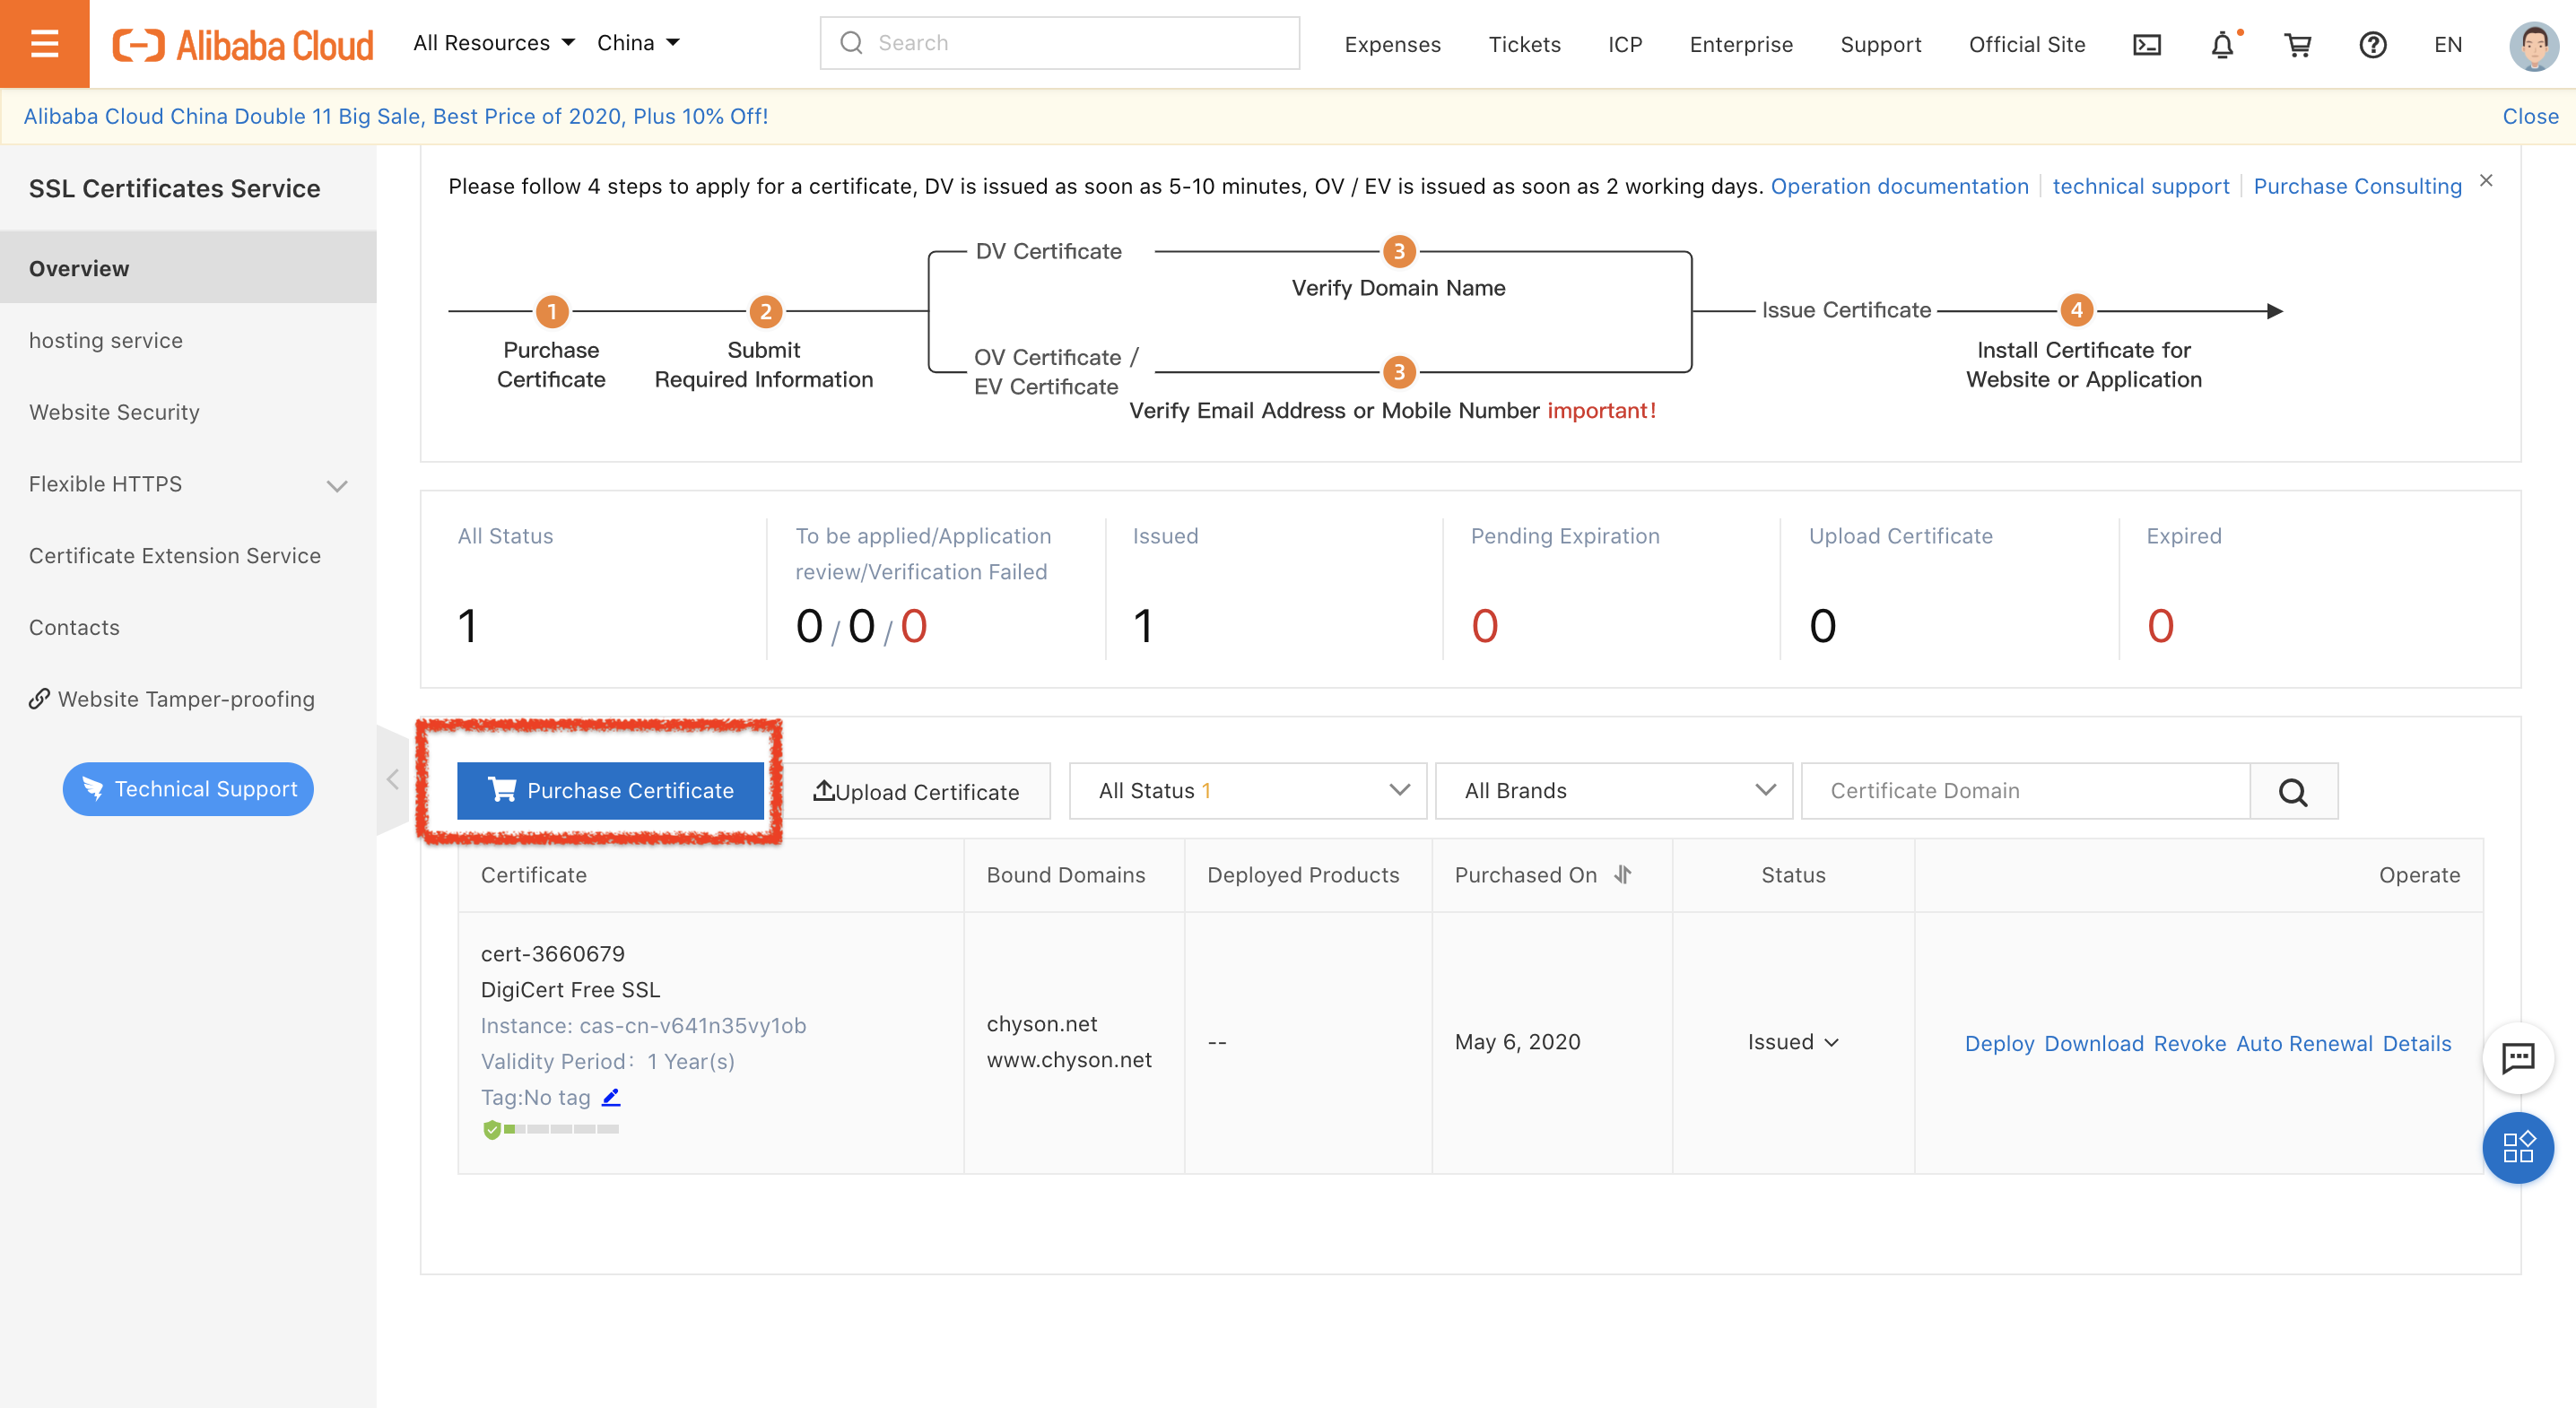
\includegraphics[width=\textwidth]{purchase-certificate.png}
  \caption{Purchase Certificate}
  \label{fig:purchase-certificate}
\end{figure}



\begin{figure}[!ht]
  \centering
  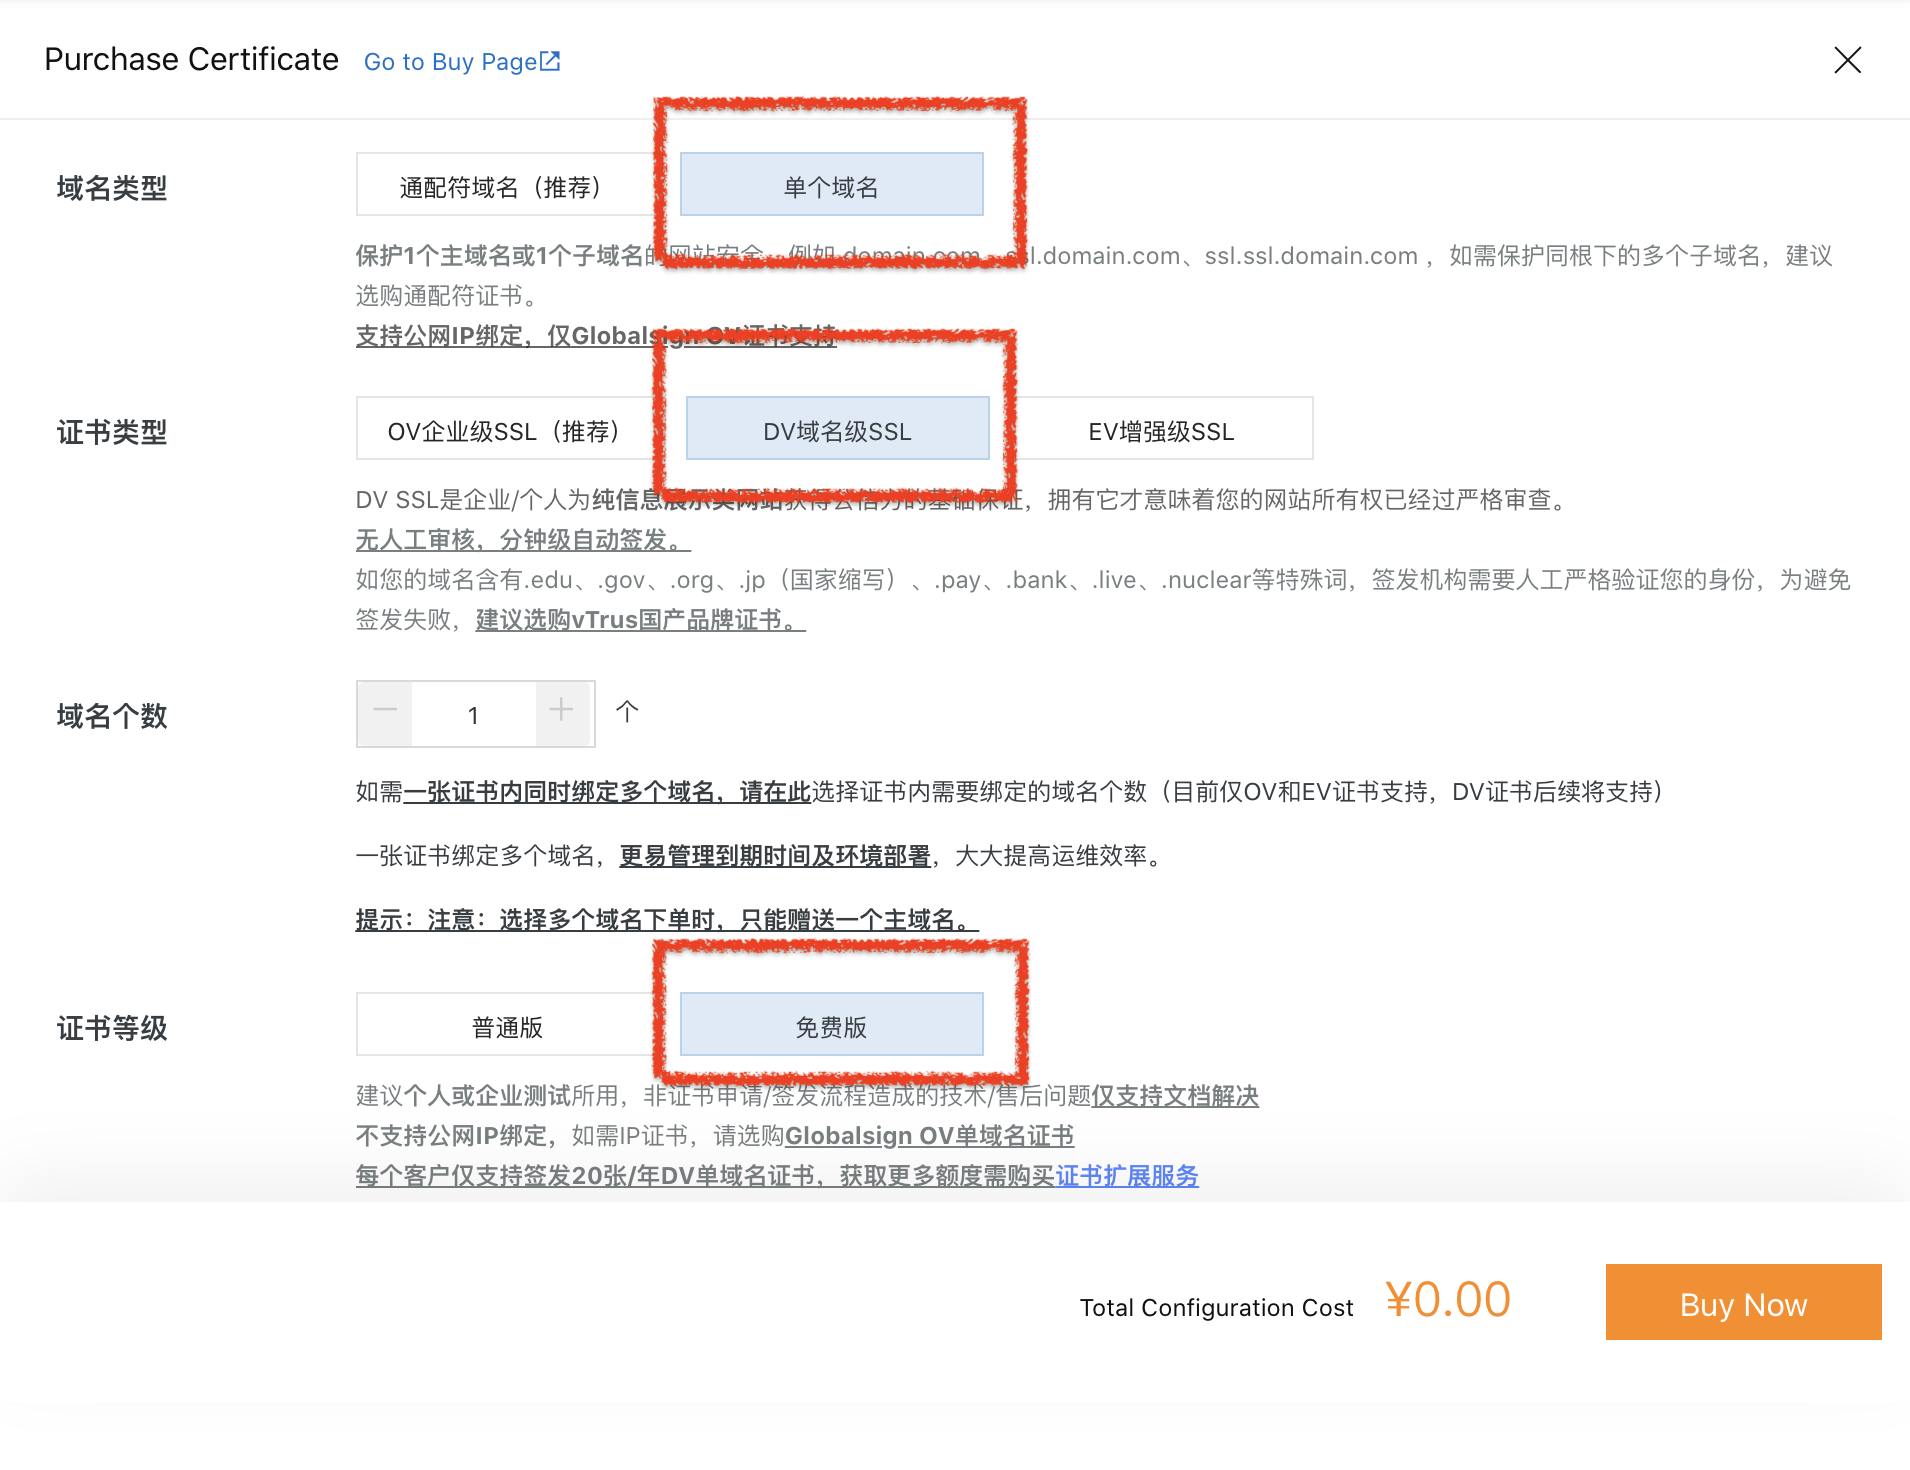
\includegraphics[width=\textwidth]{purchase-free-certificate.png}
  \caption{Purchase Free Certificate}
  \label{fig:purchase-free-certificate}
\end{figure}

\begin{tcolorbox}
  Another choice is visite the website  \url{https://letsencrypt.org/} to generate the certificate.  
\end{tcolorbox}


\section{Download your SSL certificate}
Download your SSL certificate as shown in Figure \ref{fig:download-ssl} and \ref{fig:download-ssl2}.

\begin{figure}[!ht]
  \centering
  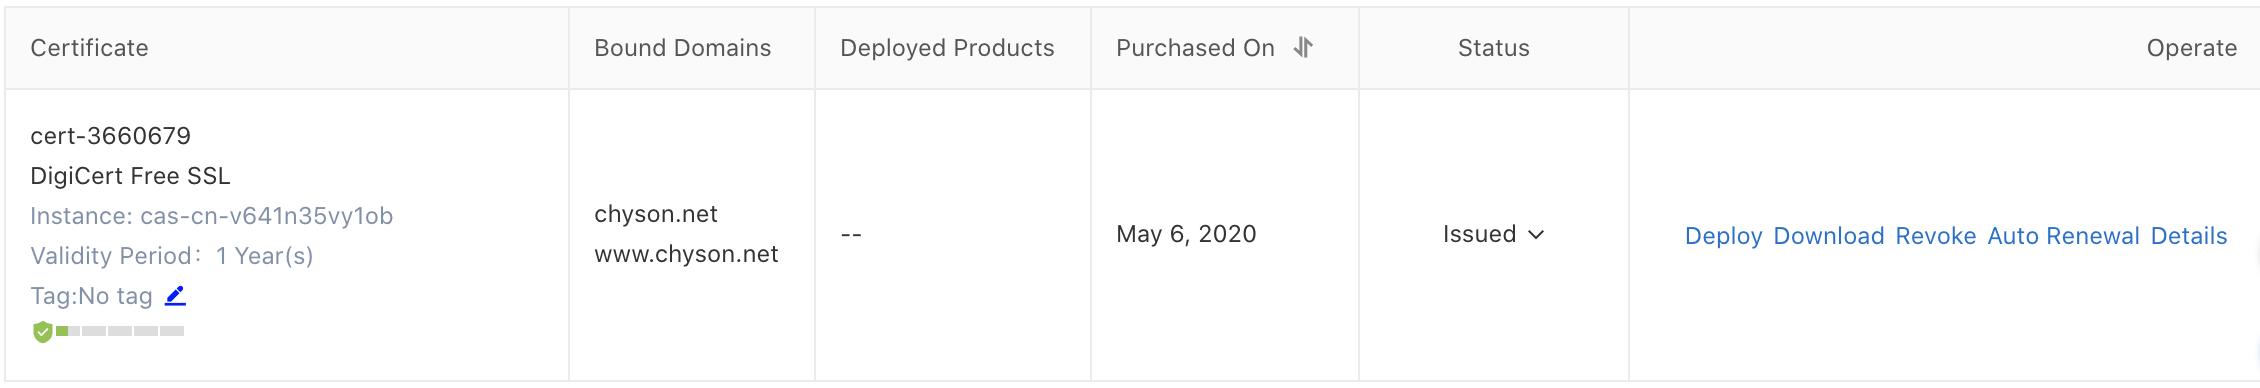
\includegraphics[width=\textwidth]{download-ssl.png}
  \caption{Download ssl}
  \label{fig:download-ssl}
\end{figure}


\begin{figure}[!ht]
  \centering
  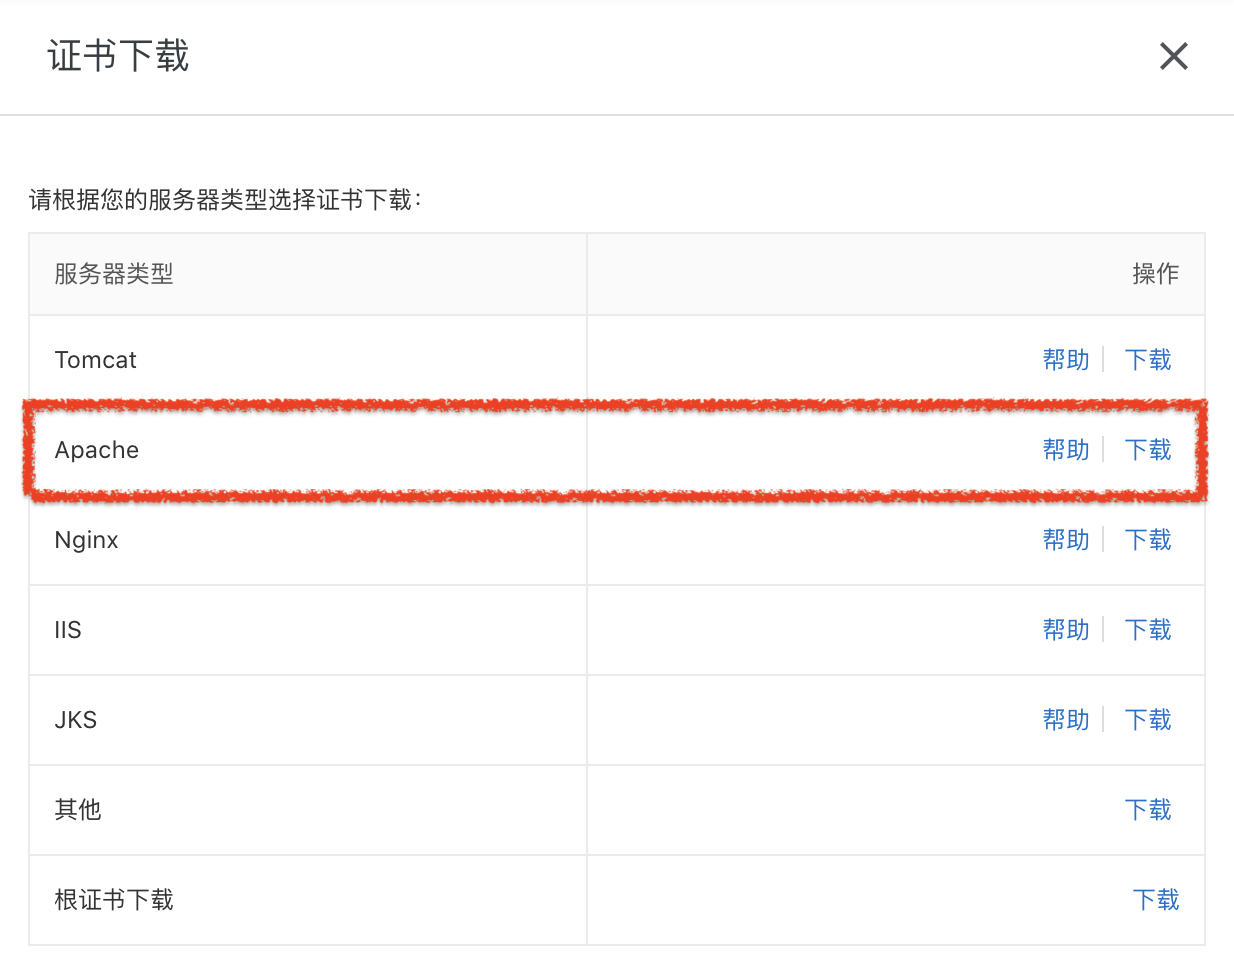
\includegraphics[width=\textwidth]{download-ssl2.png}
  \caption{Download ssl}
  \label{fig:download-ssl2}
\end{figure}

\section{Install SSL module}
\lstset{language=Sh}
\begin{lstlisting}
  dnf install mod_ssl
\end{lstlisting}

\section{Configurate SSL certificate in Apache}

Alter the configuration file \verb|/etc/httpd/conf/httpd.conf|:

\begin{lstlisting}
  LoadModule ssl_module modules/mod_ssl.so  
\end{lstlisting}

Create a directory \verb|/etc/httpd/cert| and put all you certificates in it.
\begin{verbatim}
/etc/httpd/cert/chyson.net_public.crt
/etc/httpd/cert/chyson.net.key
/etc/httpd/cert/chyson.net_chain.crt
\end{verbatim}

Alter the file \verb|/etc/httpd/conf.d/ssl.conf|:
\begin{lstlisting}
  SSLCertificateFile /etc/httpd/cert/chyson.net_public.crt
  SSLCertificateKeyFile /etc/httpd/cert/chyson.net.key
  SSLCertificateChainFile /etc/httpd/cert/chyson.net_chain.crt
\end{lstlisting}




After the configuration, restart the httpd service.
\begin{lstlisting}
  systemctl restart httpd
\end{lstlisting}


\section{Redict http to https}

Alter \verb|/etc/httpd/conf/httpd.conf|:
\begin{lstlisting}
  <Directory "/var/www/html">
  #
  # Possible values for the Options directive are "None", "All",
  # or any combination of:
  #   Indexes Includes FollowSymLinks SymLinksifOwnerMatch ExecCGI MultiViews
  #
  # Note that "MultiViews" must be named *explicitly* --- "Options All"
  # doesn't give it to you.
  #
  # The Options directive is both complicated and important.  Please see
  # http://httpd.apache.org/docs/2.4/mod/core.html#options 
  # for more information.
  #
  Options Indexes FollowSymLinks

  #
  # AllowOverride controls what directives may be placed in .htaccess files.
  # It can be "All", "None", or any combination of the keywords:
  #   Options FileInfo AuthConfig Limit
  #
  AllowOverride None

  #
  # Controls who can get stuff from this server.
  #
  Require all granted
  </Directory>
\end{lstlisting}
to
\begin{lstlisting}
  AllowOverride All  
\end{lstlisting}

Then restart the httpd service.


Create .htaccess file in \verb|/var/www/html|:
\begin{tcolorbox}
\begin{verbatim}
RewriteEngine On 
RewriteCond %{HTTPS}  !=on 
RewriteRule ^/?(.*) https://chyson.net/$1 [R,L]
\end{verbatim}
\end{tcolorbox}




\section{Cerbot}

Environment: EC2 CentOS 8, Apache

Install epel:
\begin{lstlisting}
  sudo dnf install https://dl.fedoraproject.org/pub/epel/epel-release-latest-8.noarch.rpm
\end{lstlisting}


Install snapd:
\begin{lstlisting}
  sudo yum install snapd
  sudo systemctl enable --now snapd.socket
  sudo ln -s /var/lib/snapd/snap /snap
\end{lstlisting}

Install Certbot
\begin{lstlisting}
  sudo snap install --classic certbot
  sudo ln -s /snap/bin/certbot /usr/bin/certbot
\end{lstlisting}

Run Cerbot
\begin{lstlisting}
  sudo certbot --apache
\end{lstlisting}


If  you see the problem:
\begin{lstlisting}
  Saving debug log to /var/log/letsencrypt/letsencrypt.log
Error while running apachectl configtest.

AH00526: Syntax error on line 85 of /etc/httpd/conf.d/ssl.conf:
SSLCertificateFile: file '/etc/pki/tls/certs/localhost.crt' does not exist or is empty

The apache plugin is not working; there may be problems with your existing configuration.
The error was: MisconfigurationError("Error while running apachectl configtest.\n\nAH00526: Syntax error on line 85 of /etc/httpd/conf.d/ssl.conf:\nSSLCertificateFile: file '/etc/pki/tls/certs/localhost.crt' does not exist or is empty\n")
\end{lstlisting}

Restart the httpd service and run the same command again.


If you see:
\begin{lstlisting}
  Saving debug log to /var/log/letsencrypt/letsencrypt.log
Deploying certificate
Could not install certificate
Could not reverse map the HTTPS VirtualHost to the original
Ask for help or search for solutions at https://community.letsencrypt.org. See the logfile /var/log/letsencrypt/letsencrypt.log or re-run Certbot with -v for more details.
\end{lstlisting}

Maybe the problem lies in the  mignmingli.net.conf file.
There  are extra empty line in the configuration file when you copy configuration from other document.
